\section{The GLD360 Lightning Dataset}
One could not study the global impact of LEP without a measurement of global lightning activity. Lightning is a persistent phenomenon, with an average of $\sim$ 100 strokes per second globally at any given time of day or year \citep{Brooks1925, Orville1979}.

Two primary techniques are used in the measurement of lightning distributions -- optical / infrared detection from space, and geolocation techniques using surface measurements of the guided VLF emissions, or \emph{'spherics}, which propagate in a waveguide-like manner between the Earth and the Ionosphere. 

Early optical data measurements were performed in the 1970s by the U.S. Air Force, using the Defense Meteorological Satellite Program (DMSP) satellites, which served to reveal the global distribution of lightning -- generally over land masses, and towards the equator. However, space-based optical techniques are limited to nighttime measurements, do not operate in real time, and must be performed amidst other parasitic light sources \citep{Orville1995}.

Surface-based radio detection of lightning has been in use as early as the 1920s, by magnetic direction finding (MDF) using crossed loop antennas \citep{Horner1954, Horner1957}. Such detection methods were primarily used for weather measurements before the advent of weather radar, and have seen use in early detection of forest fires \citep{Krider1980}. Terrestrial measurements have an advantage in that they can operate during both daytime and nighttime, and have detection ranges on the order of hundreds of kilometers, due to the guided propagation of 'spherics.

Large-scale detection networks became available in the early 1990s, with the U.S. National Lightning Detection Network (NLDN). NLDN provides near-real-time measurements of lightning across the continental united states using a distributed array of 114 sensors in the VLF / LF (400 Hz - 400 kHz) range. NLDN reports cloud-to-ground detection efficiencies on the order of $\sim90\%$ \citep{Nag2011}. 

Within the last decade, advances in processing techniques have fostered the ability to perform global lightning detection with a distributed array of sensors. We use the Global Lightning Dataset (GLD360), which uses a combination of time-of-arrival and direction-finding techniques, along with a precomputed waveform bank, to achieve global cloud-to-ground detection ratios on the order of $\sim{60\%}$ \citep{Said2010a}. GLD360 is a commercial service operated by \emph{Vaisala, inc.}.

GLD360 parameterizes cloud-to-ground lightning discharges by their location (latitude, longitude), and their peak current, $I_0$, as given in section \ref{section:input_power}. Figure \ref{fig:flash_rate_density} shows the annual flash rate density reported by GLD360 over a two-year period between August 2014 and April 2016; figure \ref{fig:peak_current_density} shows the average squared current density (from equation \eqref{eqn:farfield_power_td}, $S \propto I_0^2$). Within this work we take the GLD360 dataset to be the ground truth measurement of global lightning activity.

\begin{figure}[h!]
\begin{center}
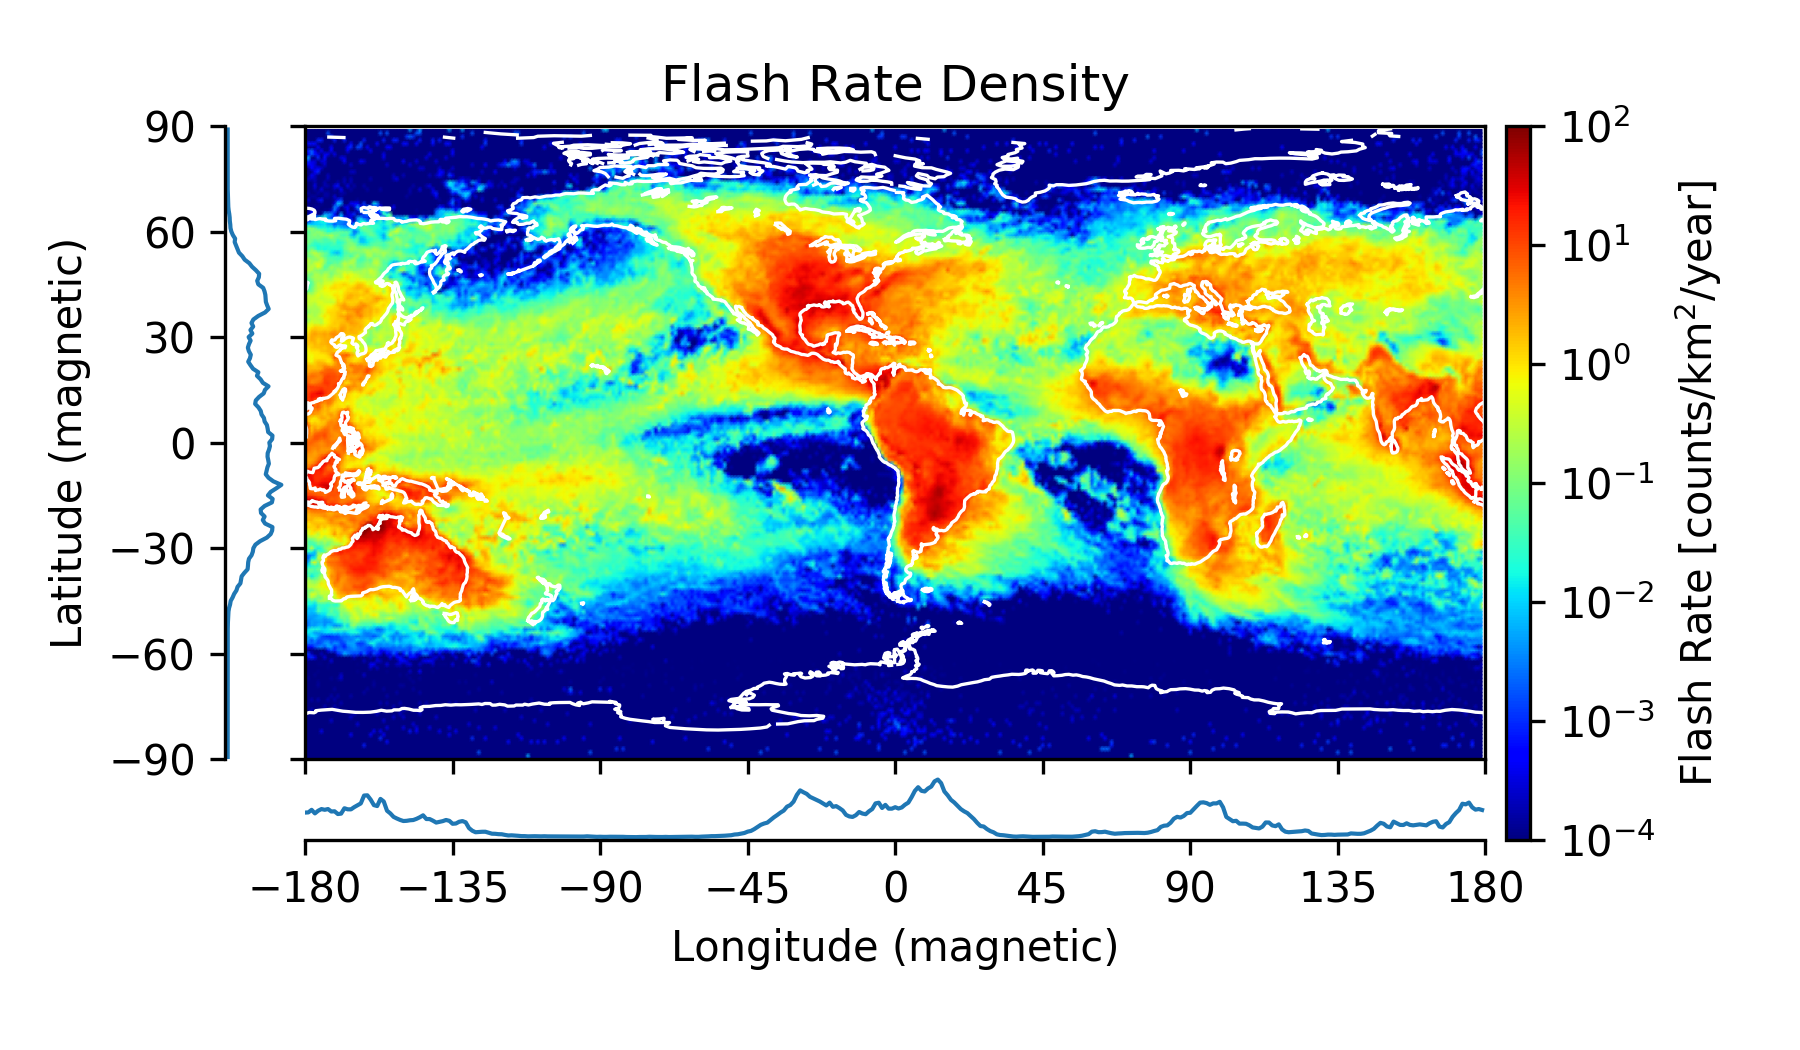
\includegraphics{figures/flash_rate_density.png}
\end{center}
\caption[Average global flash rate]{The average global flash rate distribution, as measured by the GLD360 sensor network, taken over a period between August 2014 and April 2016. The side plots show the relative density vs latitude and longitude.}
\label{fig:flash_rate_density}
\end{figure}
\begin{figure}[h!]
\begin{center}
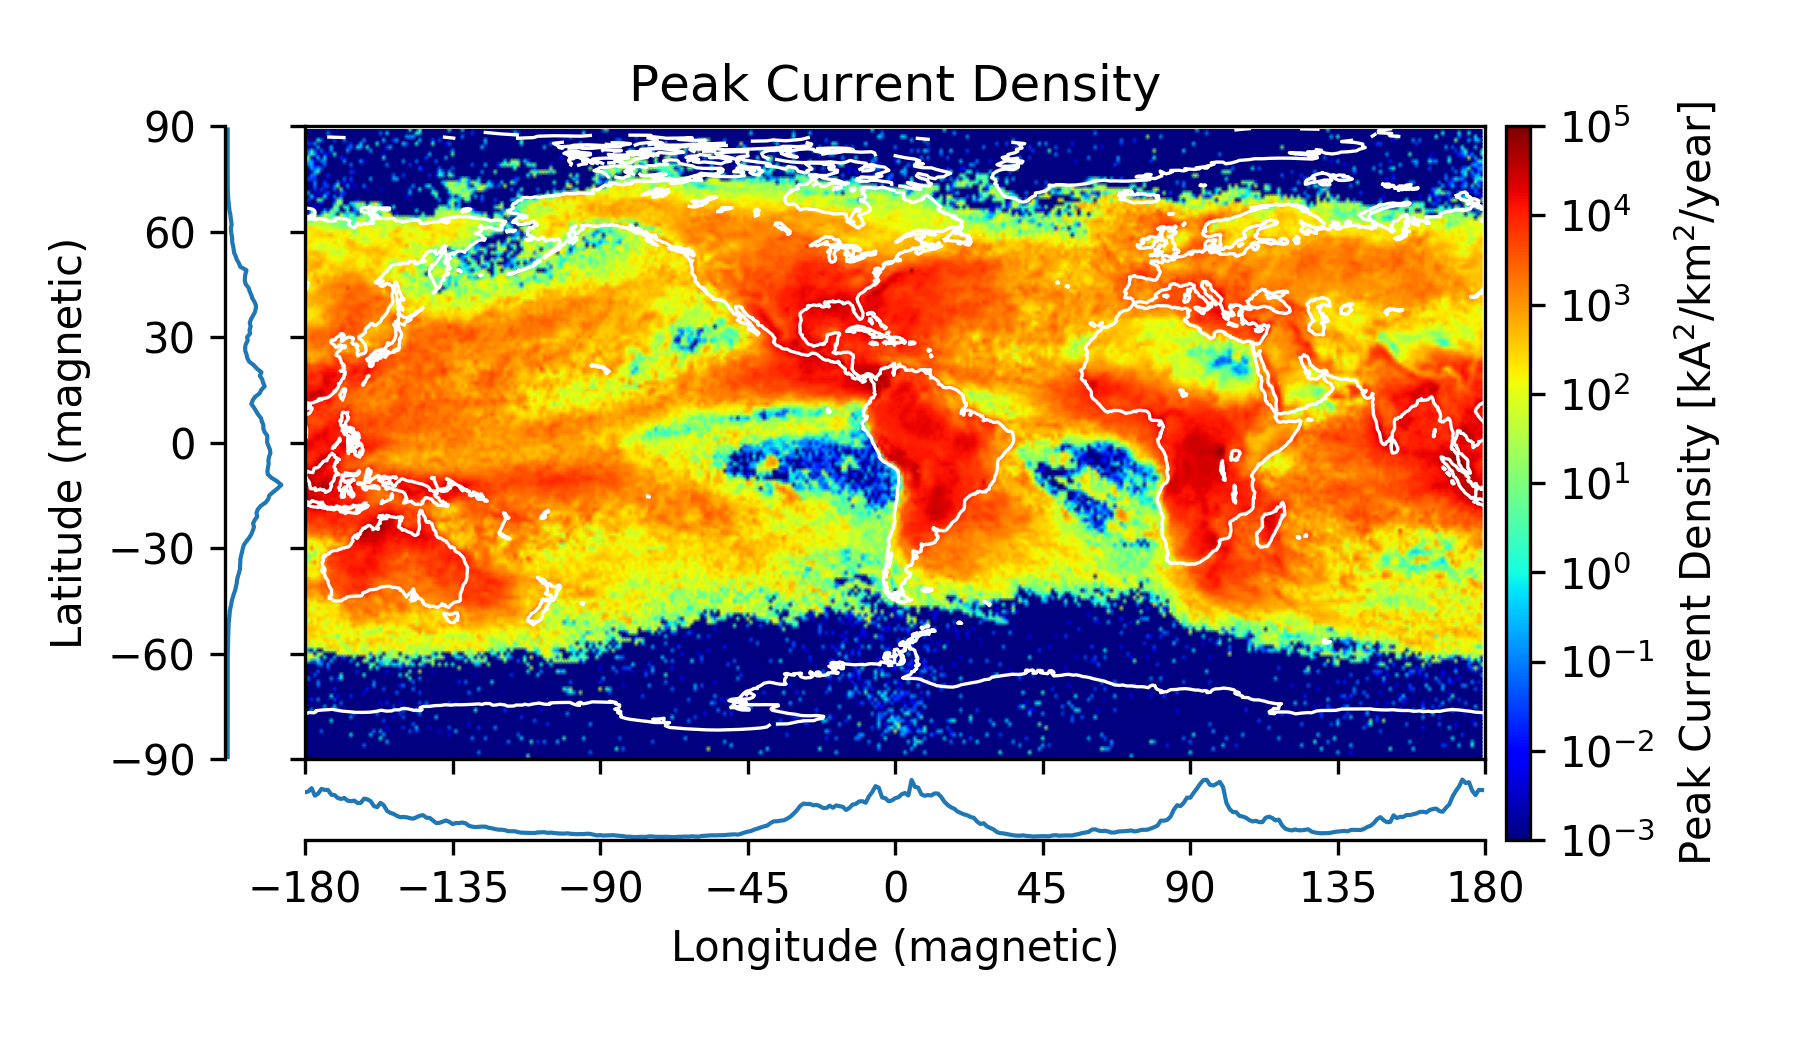
\includegraphics{figures/peak_current_density.png}
\end{center}
\caption[Average global peak current rate rate]{The average global peak current distribution, as measured by the GLD360 sensor network, taken over a period between August 2014 and April 2016. The side plots show the relative density vs latitude and longitude. While the morphology is similar to figure \ref{fig:flash_rate_density}, scaling by the average peak current indicates a possible increase in energy over the oceans.}
\label{fig:peak_current_density}
\end{figure}

